\documentclass[11pt]{article}
\usepackage[utf8]{inputenc}
\usepackage[T1]{fontenc}
\usepackage{lmodern}
\usepackage{geometry}
\usepackage{tikz}
\usetikzlibrary{arrows.meta,shapes.geometric}

\geometry{paperwidth=16cm,paperheight=3.5cm,margin=0cm}
\pagestyle{empty}
\setlength{\parindent}{0pt}

\definecolor{ctxFill}{RGB}{238,242,245}
\definecolor{ctxLine}{RGB}{155,168,179}
\definecolor{ctxText}{RGB}{38,52,67}
\definecolor{exFill}{RGB}{220,233,247}
\definecolor{exLine}{RGB}{23,54,93}
\definecolor{prFill}{RGB}{200,240,236}
\definecolor{prLine}{RGB}{8,127,140}
\definecolor{prText}{RGB}{6,79,87}

\begin{document}
\noindent
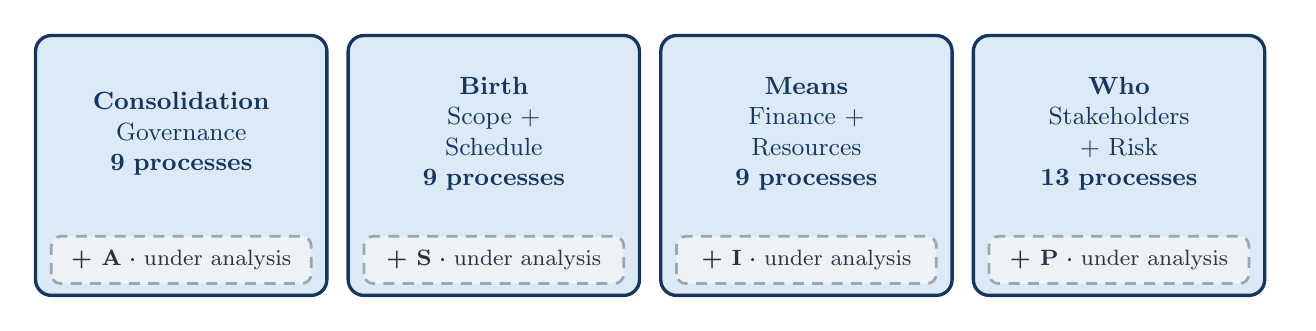
\begin{tikzpicture}[x=1cm,y=1cm,font=\small]
  \path[use as bounding box] (0,0) rectangle (16,3.5);
  \draw[fill=exFill,draw=exLine,line width=1.2pt,rounded corners=0.2cm] (0.1,0.1) rectangle (3.8000000000000003,3.4);
  \node[align=center,text width=3.4cm,text=exLine,font=\small] at (1.9500000000000002,2.15) {\bfseries Consolidation\\ \mdseries Governance\\ \bfseries 9 processes};
  \draw[fill=ctxFill,draw=ctxLine,line width=1pt,dash pattern=on 4pt off 3pt,rounded corners=0.12cm] (0.30000000000000004,0.25) rectangle (3.6,0.85);
  \node[align=center,text=ctxText,font=\footnotesize] at (1.9500000000000002,0.55) {\textbf{+ A} · under analysis};
  \draw[fill=exFill,draw=exLine,line width=1.2pt,rounded corners=0.2cm] (4.07,0.1) rectangle (7.7700000000000005,3.4);
  \node[align=center,text width=3.4cm,text=exLine,font=\small] at (5.92,2.15) {\bfseries Birth\\ \mdseries Scope +\\Schedule\\ \bfseries 9 processes};
  \draw[fill=ctxFill,draw=ctxLine,line width=1pt,dash pattern=on 4pt off 3pt,rounded corners=0.12cm] (4.2700000000000005,0.25) rectangle (7.57,0.85);
  \node[align=center,text=ctxText,font=\footnotesize] at (5.92,0.55) {\textbf{+ S} · under analysis};
  \draw[fill=exFill,draw=exLine,line width=1.2pt,rounded corners=0.2cm] (8.040000000000001,0.1) rectangle (11.740000000000002,3.4);
  \node[align=center,text width=3.4cm,text=exLine,font=\small] at (9.89,2.15) {\bfseries Means\\ \mdseries Finance +\\Resources\\ \bfseries 9 processes};
  \draw[fill=ctxFill,draw=ctxLine,line width=1pt,dash pattern=on 4pt off 3pt,rounded corners=0.12cm] (8.24,0.25) rectangle (11.540000000000001,0.85);
  \node[align=center,text=ctxText,font=\footnotesize] at (9.89,0.55) {\textbf{+ I} · under analysis};
  \draw[fill=exFill,draw=exLine,line width=1.2pt,rounded corners=0.2cm] (12.01,0.1) rectangle (15.71,3.4);
  \node[align=center,text width=3.4cm,text=exLine,font=\small] at (13.86,2.15) {\bfseries Who\\ \mdseries Stakeholders\\+ Risk\\ \bfseries 13 processes};
  \draw[fill=ctxFill,draw=ctxLine,line width=1pt,dash pattern=on 4pt off 3pt,rounded corners=0.12cm] (12.209999999999999,0.25) rectangle (15.51,0.85);
  \node[align=center,text=ctxText,font=\footnotesize] at (13.86,0.55) {\textbf{+ P} · under analysis};
\end{tikzpicture}
\end{document}
